
\section{CPFed: Communication-Efficient and Privacy-Preserving Federated Learning}

\subsection{摘要}
\paragraph{挑战:} 在联邦学习的迭代过程中, 边缘设备需要计算结果后上传到服务器进行更新. 在这个过程中, 会导致隐私泄露和\textbf{通信开销}上升. 
\paragraph{应对:} 本文提出\textbf{CPFed}, 一种通信高效和保护隐私的联邦学习方法.
\paragraph{CPFed组件:} 
\begin{enumerate}[label=(\arabic*)]  
    \item 周期性平均, 即仅在服务器上周期性平均边缘设备的本地计算结果;
    \item 高斯机制, 边缘器件在将计算结果发送到服务器之前随机扰动其本地计算结果;
    \item 安全聚合, 其中扰动的本地计算结果在发送到服务器之前同态加密. 
\end{enumerate}
\paragraph{本文工作:} 给出了CPFed的\textbf{端到端隐私保证}, 并分析了其在凸模型和非凸模型上的理论收敛速度. 通过在真实数据集上的大量数值实验, 证明了方法的有效性和效率. 
\paragraph{结果:}CPFed可以解决联邦学习中的通信效率和隐私泄露问题, 同时获得较高的模型精度.  \cite{hu2020cpfed}

\paragraph{贡献}
\begin{enumerate}
    \item 提出CPFed新型联邦学习方案CPFed, 在没有完全可信的服务器的情况下, 通过分布式数据进行高效的、差异化的私有学习. 
    \item CPFed通过允许部分设备在每次迭代时参加培训并定期与服务器通信来减少通信数量. 
    \item 在不降低模型精度的情况下, CPFed通过集成安全聚合和不同隐私技术, 严格保护每个设备的数据隐私. 
    \item 零集中的差异隐私密切考虑CPFed的端到端隐私损失. 
    \item  对强凸和非凸损失函数进行CPFed的收敛分析, 并基于真实数据集进行广泛的评估. 
\end{enumerate}

\subsection{背景介绍}

\subsubsection{挑战}

\paragraph{通信开销}
虽然联邦学习中边缘设备和服务器只传递模型更新, 但是可能包含(深度神经网络的)数亿个参数, 而且需要多次迭代才能获得较高精度模型. 边缘设备大多资源受限(带宽有限,特别是上行传输时).
\paragraph{隐私泄露}
只传输模型更新不足以保证隐私安全. 例如难以抵御重构攻击和成员推理攻击.


\subsubsection{差分隐私DP}
\paragraph{$(\varepsilon,\delta)-DP$} 
随机算法$\mathcal{M:D \to R}$, 其中定义域$\mathcal{D}$, 值域$\mathcal{R}$
\begin{equation}
    Pr [ \mathcal{M}(D) \in S ] \leqslant \exp(\epsilon c) \cdot Pr [ \mathcal{A(D_2)} ] \in S  + \delta 
\end{equation}

其中,$D, D^{'} \in \mathcal{D}$为两个两个数据集, 输出 $S \in \mathcal{O}$, $\varepsilon$称为预定隐私.
可以在输出加上高斯噪声.

\paragraph{$\rho$零集中DP($\rho-\text{zCDP}$)}
$\rho-\textbf{zCDP}$具有紧密的组合约束, 更适合分析迭代算法的端到端隐私损失. 
$\rho-\textbf{zCDP}$满足
\begin{equation}
    \mathbb{E}[e^{(\alpha-1)Z}] \leqslant e^{(\alpha -1)\rho}
\end{equation} 
其中\subparagraph{隐私损失} 
\begin{equation}
    Z := \log \frac{Pr[\mathcal{M}(D)]=o}{Pr[\mathcal{M}(D^{'})]=o} 
\end{equation}

其中$o \in \mathcal{R}$
$\rho-\textbf{zCDP}$的性质

\begin{figure}[ht]
    \setlength{\abovecaptionskip}{0.1cm}
    \centering    
    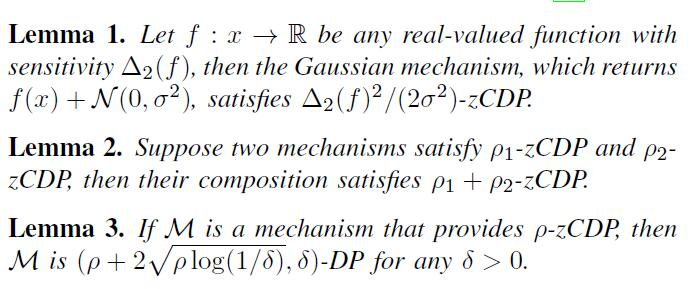
\includegraphics[width=0.7\textwidth]{CPFed/zCDPLemma.jpg}
    \caption{$\rho-\textbf{zCDP}$性质}
\end{figure}

\subsection{系统建模}
\subsubsection{联邦学习系统}
联邦学习吸引包含n个客户机, 每个有$m$条数据, 表示为$D_i = {\xi^i_1, \ddot,\xi^i_m}$
\textbf{客户机目标}是训练一个共同模型 $\theta \in \mathbb{R}^d$, 即最小化所有本地数据的联合最小经验损失.
\begin{equation}
    \min_\theta f(\theta) := \frac{1}{n} \sum^n_{i=1}f_i(\theta) \ \  \text{其中},f_i(x) := \frac{1}{m}\sum_{\xi\in D_i} l(\theta , \xi ) 
\end{equation}
其中$f_i$是客户机$i$的局部目标函数,$l(\theta; \xi)$是模型$\theta $在点$\xi\in D_i $处的损失.

\subsubsection{威胁}
本文假设对手有两类:
\begin{enumerate}
    \item “诚实但好奇”的中央服务器或客户机. 中央服务器将忠实地遵循设计的培训协议, 但会对客户机的私有数据感到好奇, 并可能从共享的消息中推断真实信息. 
    \item 被动的攻击者:在训练中窃听共享消息,但不主动攻击.
\end{enumerate}


\subsubsection{目标}
设计一个方案使客户机以低成本通信成本训练模型并保证隐私.

\subsection{CPFed}

\subsubsection{提高通信效率--周期平均}
\paragraph{问题} 起初方法--分布式SGD,由于通信速度比本地慢数个数量级,且联邦学习通常设备过多,导致总体效率低下.

\paragraph{改进方法}
同时减少通信轮的数量和每轮涉及的客户端, 如图2所示. 在我们的方法中, 服务器首先均匀随机地选择一组客户端, 然后让选中的客户端执行多次迭代以最小化本地目标, 然后再将其本地计算结果发送给服务器. 
简单来说,就是分组分级策略,相当于联邦的每个州继续往下分为各县. 各县先统计好本地数据再提交. 这和小批量随机梯度下降的思想相似.
在第$t$轮迭代是,一组$r$个客户机$\Omega_t$通过$\tau$次局部训练预先训练模型$\theta^t$,
用$\theta_i^{t,s}$表示第$t$轮迭代的第$s$轮局部迭代的客户机$i$的局部模型.

\begin{equation}
    \theta^{t,s+1}_i= \theta_i^{t,s}- \eta g(\theta_i^{t,s})
\end{equation}
其中 $g(\theta_i^{t,s}) := \frac{1}{B} \sum_{X_i} \nabla l(\theta_i^{t,s,\xi)}$表示基于一批B条数据$X_i$的小批量随机梯度下降计算. 

$\tau$轮迭代后,服务器共享模型更新为 
\begin{equation}
    \theta^{t+1}=\frac{1}{r} \sum_{i\in \Omega_t} \theta_i^{t,\tau} 
\end{equation}
 

\begin{figure}[ht]
    \
    \setlength{\abovecaptionskip}{0.1cm}
    \centering    
    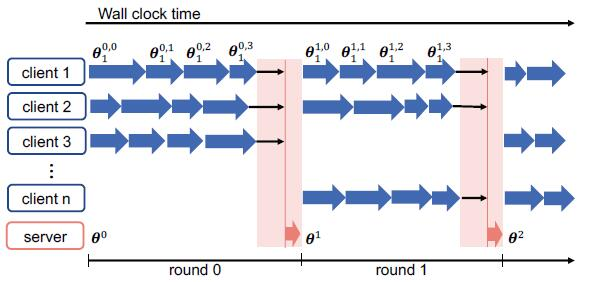
\includegraphics[width=0.7\textwidth]{CPFed/communication-reduction.jpg}
    \label{communication-reduction-strategies}
    \caption{$\tau=4,r=3 $时的通信减少策略}
\end{figure}
 
\subsubsection{防止隐私泄露--DP}

\paragraph{问题} 通信减少策略不能阻止更高级的攻击(推断)
\paragraph{设计目标} $\theta_t$和${\theta_i^{t, \tau}}_{i\in\Omega_t}$包含隐私数据,通过DP防止两种隐私泄露
\paragraph{设计}

\begin{equation}
    \theta_i^{t,s+1}= \theta_i^{t,s}- \eta (g(\theta_i^{t,s})) + b_i{t,s} 
    \label{local_iter}
\end{equation}
其中 $b_i{t,s}$是第$t$轮迭代的第$s$次局部迭代时取样自分布$N(0,\sigma^2 \mathbf{1}_d)$的高斯噪声

\paragraph{结果} 由于DP的后处理特性, 局部模型的和$\theta^{t+1}$ 为客户端保留和本地模型{\color{red}相同级别的DP保证 }

\subsubsection{提升模型精确度--安全集聚}

\paragraph{问题} 由于使用高斯机制的差分隐私,模型精确度将会下降
\paragraph{分析} 服务器只需知道本地模型的平均值,可以隐藏单个本地模型,减少客户端隐私损失
\paragraph{设计目标} 设计基于秘密共享的协议,安全聚合应能够达到以下目标
\begin{enumerate}[label=(\arabic*)]  
    \item 隐藏客户端的单个消息
    \item 恢复每一轮随机客户端的单个消息总和, 
    \item 使参与的客户端的通信成本较低. 
\end{enumerate}


\paragraph{设计}
提出的安全协议包括以下两个步骤:
\begin{enumerate}[label=(\arabic*)]  
    \item 加密上传:$\Omega_t$中的客户机上传自己的加密本地模型$\{ c_i^t\} I{i\in \Omega_t}$到服务器
\item 解密:服务器解密来自客户机组$\Omega_t$的消息和. 

\end{enumerate}

 
安全协议的基本思想是在明文中添加随机数$r_i^t$来保护客户机$i$的信息$p_i^t$.即$c^t_i = p^t_i +r^t_i$,难点在于使所有客户机的$r^t_i$和为0, 消除随机数的影响. 但是这要求客户机相互通信,这会导致低效通信.

解决方案是引入伪随机函数(PRF)$G$

PRF $G$要求在初始化和第$t$轮迭代时客户机$i$和$j$统一随机数种子$seed_{i,j}$,,并且每轮循环输出不同的伪随机数$G(seed_{i,j},t)$. 这样每次客户机无需经过和其他客户机交互便可计算出$r_i^t$, 便可降低通信开销.

\begin{figure}[ht]
    \
    \setlength{\abovecaptionskip}{0.1cm}
    \centering    
    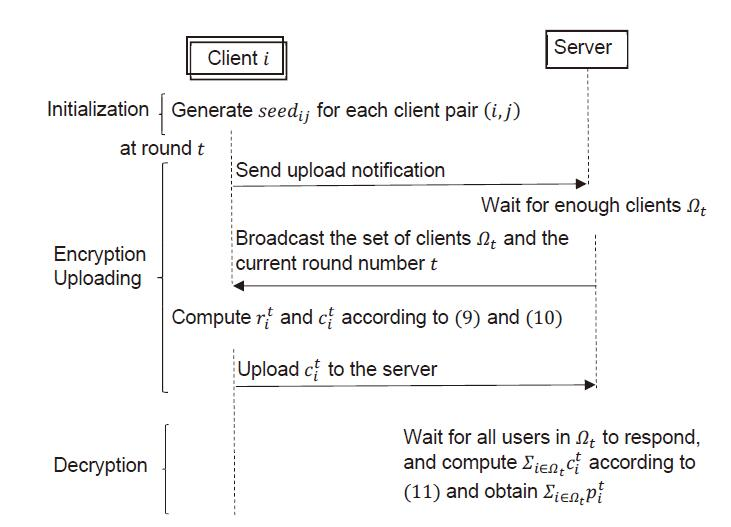
\includegraphics[width=0.7\textwidth]{CPFed/secure-aggregation.jpg}
    \caption{CPFed中的高效安全聚合协议}
\end{figure}
 
\paragraph{加密过程}
在客户机组$\Omega$中,客户机$i \in \Omega_t$计算密钥
\begin{equation}
    r_i^t= \sum_{j \in \Omega_t \backslash \{i\}}(r_ij^t-r_ji^t)
\end{equation}

其中 $r_ij^t=G(seed_{i,j})$客户机$i,j$共知. 客户机$i$的密文为

\begin{equation}
    c_i^t=p_i^t+ r_i^t 
\end{equation}

\paragraph{解密过程}

\begin{equation}
    \sum_{i \in \Omega_t} c_i^t=   \sum_{i \in \Omega_t} p_i^t +   \sum_{i \in \Omega_t}   \sum_{j \in \Omega_t \backslash\{i\}} (r_ij^t-r_ji^t) = \sum_{i \in \Omega_t} p_i^t 
\end{equation}

\subsubsection{CPFed总体方案}
\begin{figure}[ht]
    \setlength{\abovecaptionskip}{0.1cm}
    \centering    
    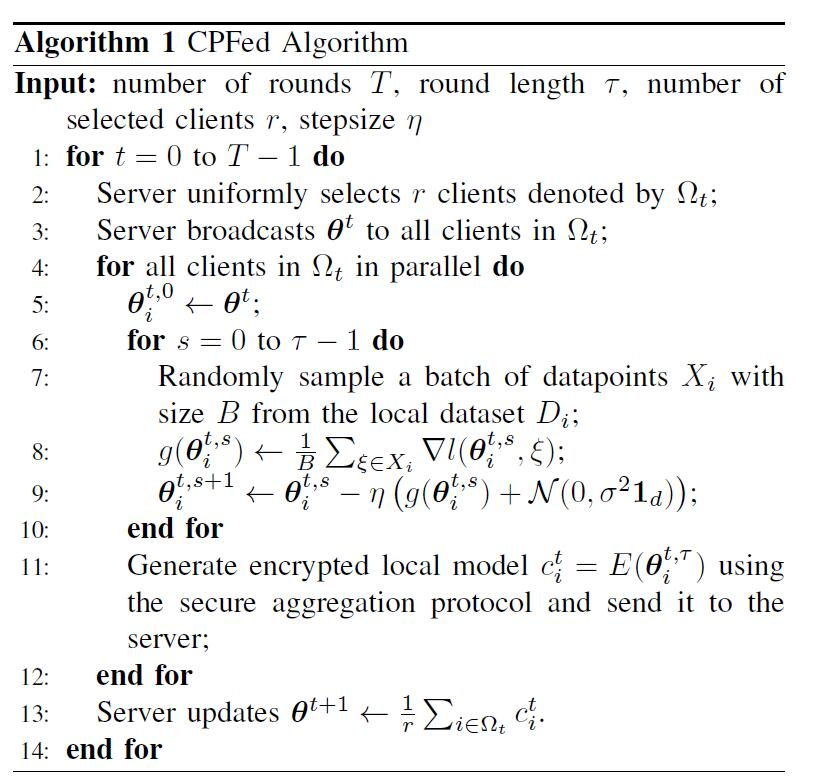
\includegraphics[width=0.7\textwidth]{CPFed/CPFed_Algorithm.jpg}
    \label{CPFed_algorithm}
\end{figure}

CPFed由$T$轮通信迭代组成,每一轮迭代选择一组客户机$\Omega_t$, 其数据集为$\mathcal{D}_i$使用\ref{local_iter}进行$\tau$次局部迭代, 其中每组客户机每轮进行初始化共同的模型. $\tau$轮局部迭代后, 客户机组$\Omega_t$上传加密模型$E(\theta_i^{t,\tau})$,服务器对这些加密信息进行聚合.

\subsection{隐私分析}

\paragraph{Corollary推论1} 第$t-th $轮的第$s$次局部迭代时, 客户$i$的随机梯度$g(\theta_i^{t,s})$的灵敏度以$2L/B$为界. 

\paragraph{Lemma 4 } 
上传的本地模型总和的敏感度$\sum_i \in \Omega_t \theta^{t, \tau}_i$
以$2 \eta \tau L/B$为界. 

通过Lemma 1和4, 可得每轮的zCDP保证

\begin{theorem}
如果算法1中的高斯噪声$b_i^{t,s}$取样与$N(0, \sigma^2 \mathbb{1}_d)$
, 那么算法1经过T轮可以为每个客户机达到$(\epsilon,\delta)-DP$, 其中 
\begin{equation}
    \epsilon = \frac{2T\tau L^2}{n B^2 \sigma^2}+ 2 \sqrt{\frac{2T\tau L^2 }{nB^2\sigma^2} \log\frac{1}{\delta}} 
\end{equation}
\end{theorem}

\subsubsection{收敛性分析}

\begin{figure*}[!ht]
    \setlength{\abovecaptionskip}{0.1cm}
    \centering    
    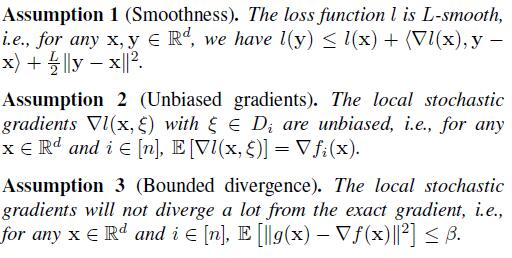
\includegraphics[width=0.7\textwidth]{CPFed/Assumption123.jpg}
    \label{assumption123}
\end{figure*}

假设2中, 无偏差梯度保证随机梯度算法的随机性不影响结果的准确性. 
假设3保证局部随机梯度相差在一定范围内, 即忽略一些客户机偏离正常值
过远的梯度数据. 这些都是联邦学习的常见假设. 
由假设2和假设3, 便可得出引理5: 局部随机梯度的方差有界, 且与精确梯度相差不大.



\begin{figure*}[!ht]
    \setlength{\abovecaptionskip}{0.1cm}
    \centering    
    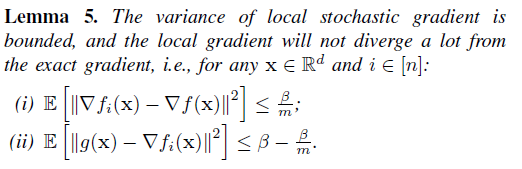
\includegraphics[width=0.7\textwidth]{CPFed/Lemma5.png}
    \label{Lemma5}
\end{figure*}
\newpage
\subsubsection{虚拟更新规则}

定义$\Theta^k, G^k,B^k \in \mathbb{R}^{d \times n} \text{其中} k =0, \dots  K$连接所有局部模型, 梯度, 和噪音
\begin{figure*}[!ht]
    \setlength{\abovecaptionskip}{0.1cm}
    \centering    
    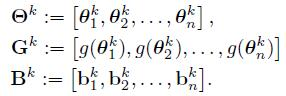
\includegraphics[width=0.4\textwidth]{CPFed/virtualUpdate.jpg}
    \label{virtualUpdate}
\end{figure*} 

\begin{figure*}[!ht]
    \setlength{\abovecaptionskip}{0.1cm}
    \centering    
    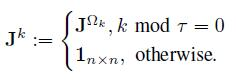
\includegraphics[width=0.5\textwidth]{CPFed/Jk.jpg}
    \label{Jk}
\end{figure*}

\textbf{连接?}


$k \mod \tau =0$意思是每轮迭代结束,进行平均,其余迭代时$J^k= 1_{n \times n} $表示该值无影响.
CPFed 的一般更新规则可以表示为

$$ \Theta^{t+1} =( \Theta ^k - ]eta ( G^k+B^k)) J^k$$

第$k$次迭代的平均模型可表示为

$$ \frac{\Theta^{k+1} \mathbf{1}^k}{r} =\frac{\Theta^k \mathbf{1}^k}{r}- \eta (\frac{G^k \mathbf{1}^k}{r} +\frac{B^k\mathbf{1}^k}{r} )$$


\textbf{安全聚合不会更新本地模型的总和}.

上式可重写为
\begin{figure*}[!ht]
    \setlength{\abovecaptionskip}{0.1cm}
    \centering    
    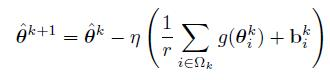
\includegraphics[width=0.6\textwidth]{CPFed/equation16.jpg}
\end{figure*}

\begin{figure*}[!ht]
    \setlength{\abovecaptionskip}{0.1cm}
    \centering    
    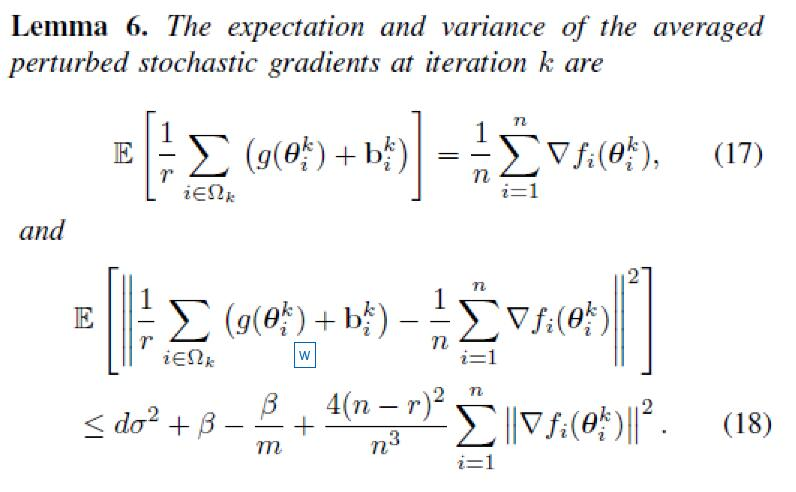
\includegraphics[width=0.7\textwidth]{CPFed/Lemma6.jpg}
    \label{Lemma6}
\end{figure*}

\begin{theorem}
(凸损失的CPFed收敛性)
对于CPFed算法, 假设迭代总次数为$K= T\tau$的次数, 其中$T$为通信轮数, 而n为轮长. 在假设1-4的条件下, 如果学习率满足$5\eta L +20 \tau ^2\eta^2 L^2 \leqslant 1$, 并且所有的客户端初始化在同一个点 $\theta ^0 \in \mathbb{R}^d$, 那么经过K次迭代后, 期望最优性间隙有界如下:
\begin{equation}
  \mathbb{E} \left[  \frac{1}{K} \sum_{k=0}^{K-1}f(\theta^k)-f^\star \right]\leqslant
  \frac{(1-n\lambda)}{K \eta \lambda}  (f(\theta^0)-f^\star (1-n)
  +H(\tau,\sigma^2)
\end{equation}
,其中$H(\tau,\sigma^2) := \eta L /2 \lambda (4 \eta L(\eta L(\tau -1)(2 \tau-1)+1) (d \sigma^2+\beta - \beta /m ))$, $\xi^2$为小批量随机梯度的方差界, 其中, $\sigma^2$为高斯噪声的方差, L为梯度的Lipschitz常数, $\lambda$ 是为强凸性常数, m为局部数据集的大小

\end{theorem}

\begin{theorem}
(CPFed对非凸损失的收敛性). 
对于CPFed算法, 设总送代次数$K=T\tau$, 其中$T$为通信轮数, 而$d$为轮长. 
在假设1-3的条件下, 如果学习率满足$5\eta L +20 \tau ^2\eta^2 L^2 \leqslant 1$, 并且所有的客户端初始化在同一个点 $\theta ^0 \in \mathbb{R}^d$, 那么经过K次迭代后, 期望最优性间隙有界如下:
\begin{equation}
  \mathbb{E} \left[  \frac{1}{K} \sum_{k=0}^{K-1}f( \| \hat{\theta}^k) \|^2  \right]\leqslant 
  \frac{2(f(\theta^0)- f^\star)}{ \eta K} + P(\tau, \sigma^2) 
\end{equation}
, 其中$P(\tau,\sigma^2) := \eta L /2 \lambda (4 \eta L(\eta L(\tau -1)(2 \tau-1)+1) (d \sigma^2+\beta - \beta /m ))$, $\xi^2$为小批量随机梯度的方差界. 其中, $\sigma^2$为高斯噪声的方差, L为梯度的Lipschitz常数, m为局部数据集的大小.
\end{theorem}   



%具体证明另外手写.

\subsection{实验}

\subsubsection{实验装置}
\paragraph{数据集} Adult dataset 48842个样本 14个数字特征(年龄,阶级,种族,性别等)和分类特征(收入). 原始数据分配给16台设备.
\paragraph{学习任务} 训练一个逻辑回归分类器和一个3层神经网络分类器(使用ReLU激活函数)

\paragraph{基准} DP-SGD, 在 DP-SGD中, 每个设备在每个集聚阶段只进行一步随机梯度下降对局部模型进行更新, 每次更新模型时加入高斯噪声后再发送. 

\paragraph{超参数} 80\%的数据用于训练,10\%用于测试,10\%用于验证. Lipschitz常数设为1, 隐私失效概率$=10^{-4} $客户端数$r=10$.

\subsubsection{CPFED的收敛性}
实验参数

逻辑回归
$ \sigma = {10^{-5},10^{-4},10^{-3}}, \tau=\{1,5,10,40\}$
神经网络 
$ \sigma = {10^{-4},10^{-3},5 \times 10^{-3},10^{-3}}, \tau=\{1,5,10,40\}$

\begin{figure*}[!ht]
    \setlength{\abovecaptionskip}{0.1cm}
    \centering    
    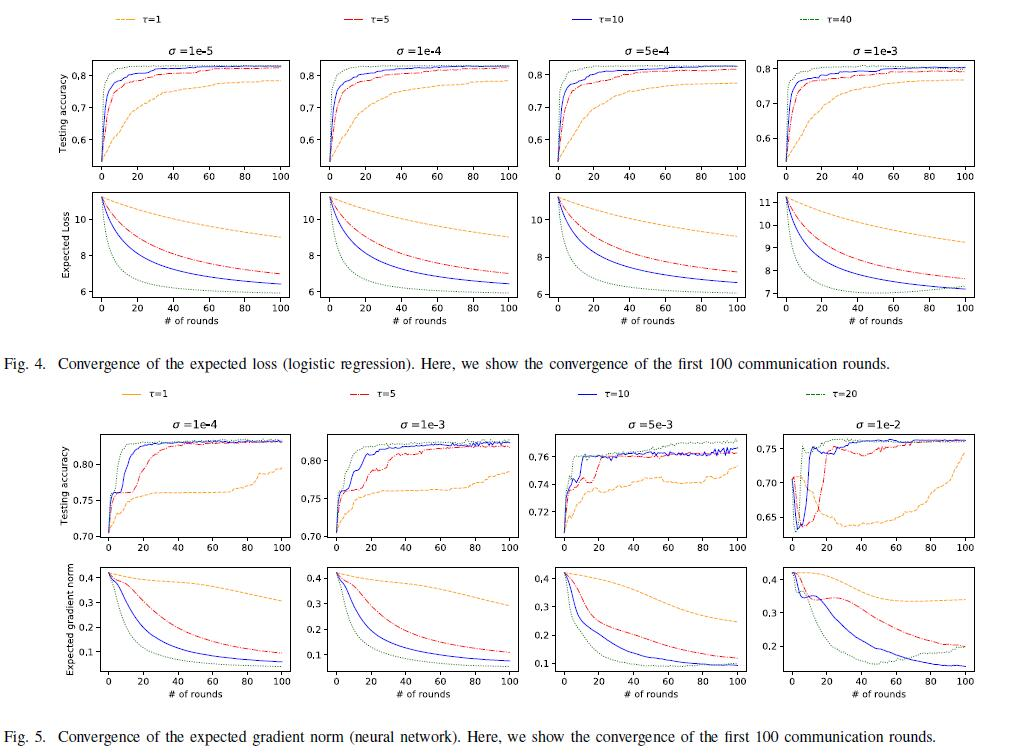
\includegraphics[width=\textwidth]{CPFed/experiment45.jpg} first proposed the concept of deep learning with differential privacy (DP), providing an evaluation criterion for privacy guarantees
\end{figure*}

\begin{figure*}[!ht]
    \setlength{\abovecaptionskip}{0.1cm}
    \centering    
    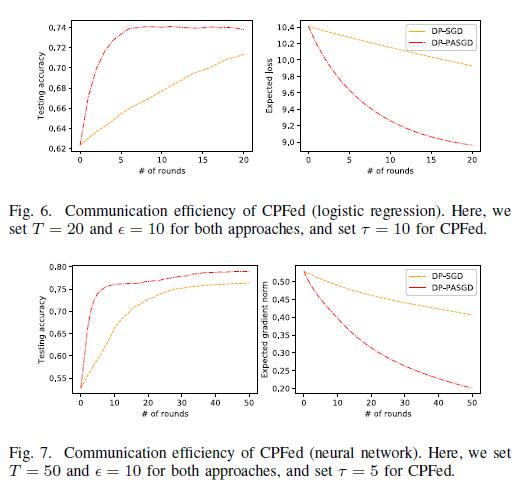
\includegraphics[width=0.8\textwidth]{CPFed/experiment67.jpg}
\end{figure*}

对于logistic回归分类器, 测试准确率和预期损失一般会先急剧下降后缓慢下降. 随着噪声级的增大, logistic回归的期望训练损失收敛到一个更高的界, 测试精度下降, 这与CPFed的收敛特性一致, 其中, 较大的噪声级(index)意味着较大的收敛误差. 对于所有的噪声设置, 随着局部送代次数的增加, 预期损失在开始时下降的更剧烈, 并且到达一个更高的平稳点, 这与CPFed的收敛特性一致, 即较大的收敛系数意味着较大的收敛误差. 

神经网络分类器也有类似的趋势. 当$\sigma=10^{-2}$时当噪声进入系统时, 测试精度会从初始值迅速下降, 然后随着计算量和通信量的增加而增加. 说明加噪声过大影响精确度.

\paragraph{通信效率比较} CPFed与基准方法DP-SGD的通信效率进行比较, CPFed比DP-SGD收敛更快, 比DP-SGD获得更高的精度和更低的期望梯度范数. 无论在凸还是非凸情况下, CPFed都比DP-SGD实现了更高的通信效率. 因为CPFed可以在多台机器上进行多步梯度更新,模型能更快收敛.

